%%%%%%%%%%%%%%%%%%%%%%%%%%%%%%%%%%%%%%%%%%%%%%%%%%%%%%%%%%%%%%%%%%%%%%%%%%%
%
% ML Presentation Paper 
% Jeremy Lao/John Reynolds
% JJL359, JR4716
%%%%%%%%%%%%%%%%%%%%%%%%%%%%%%%%%%%%%%%%%%%%%%%%%%%%%%%%%%%%%%%%%%%%%%%%%%%

\documentclass[11pt]{article}

% AMS packages:
\usepackage[fleqn]{amsmath}
\usepackage{amsmath, amsthm, amsfonts}

% Document Formatting Packages:
\usepackage{hyperref}
\usepackage[margin=1in]{geometry}
\usepackage{graphicx}
\usepackage{caption}
\usepackage{subcaption}
\usepackage{float}
\newcommand{\vertSpace}[1]{\vspace{3mm}}


%----------------------------------------------------------------
\title{Predicting FOMC Actions using NLP; Assesing the impact of matrix sparsity and regularization}
\author{
        Jeremy Lao - jjl359 \\
        NYU Computer Science \\
            \and
        John Reynolds - jr4716 \\
        NYU Computer Science \\
}

\begin{document}
{\setlength{\mathindent}{0cm}
\maketitle

\abstract{\textit{The Federal Open Market Committee (FOMC) meets throughout the year to set the target Federal Funds rate.  The Federal Funds rate is one of the primary monetary policy tools, and it impacts the cost of borrowing money globally.  This paper explores ML and NLP methods, examines the impact of matrix sparsity from NLP methods and regularization from ML models, to predict the potential outcome of an upcoming FOMC using past FOMC statements and meeting minutes to train ML and NLP models.}}

\section{Introduction}
In this paper we use Natural Language Processing (NLP) and Machine Learning (ML) methods to predict Federal Open Market Committee (FOMC) rate actions (hold or change) using text from FOMC meeting minutes, Board of Governors speeches, and FOMC post-meeting statements.  \vertSpace

 
For this analysis we used 713 separate documents (rougly 1.6 Million Words) and 148 Fed Decisions for our data set.  We employ the NLP bag-of-words model for our analysis.  Bag-of-words models have high dimensionality, meaning the space is extremely sparse with a large amount of features leading to a sparse feature matrix.  We found in our analysis that some of the feature matricies contained over two billion elements with as little as $0.25\%$ of the elements containing a non-zero value.  \vertSpace


Due to these modelling challenges, the analysis and techniques we used address the issue of features being magnitudes larger than the label size ($p>>n$), and the extreme sparsity in the feature matrix.  In order to determine the appropriate model, n-gram size, and model parameters, we created a simulator to detect positive or negative sentiment from randomly generated text.  \vertSpace 


Our model simulator found that as the number of sentiment words increased, the prediction accuracy approached close to 1.0 with high F1 scores.  For the study the analysis hones in on the mix of distributions containing hawkish or dovish (positive-action) words.


\subsection{git repository for project}
\url{https://www.github.com/jrrpanix/ML9}

\section{Objectives}
\begin{enumerate}
\item Given the proliferation of robust open-source ML and NLP packages, we were driven to understand the characteristics of the feature matrix output (i.e., document-term matrix) from the text processing functions (i.e., CountVectorizer) analyzing the number of features, matrix sparsity, and matrix norm generated from utilizing packages functions.
\item Assess the effeiveness of Multinomial Niave Bayes and Logistic Lasso applied to problems where the feature size is orders of magnitues larger than the label size ($p>>n$).
\item Determine whether ML and NLP methods can be used to predict FOMC action (no change or a change in the base rate) using FOMC statements, minutes, and Board of Governors speeches.
\item Measure model performance on F1 scores because $70\%$ of the actions over the nineteen year period we are measuring are ``no action''.  F1 scores ensure that the accuracy of the model is not based purely on a naive ``no action'' guess, which in the best case would give a $70\%$ model accuracy.
\item Create scraping and cleaning tools to assemble a corpus of documents containing Speeches, Statements, Minutes and Actions from the Federal Reserve.
\end{enumerate}

\section{Methodology}

\subsection{Data}

The time frame of our study covered 2000 to 2018. We primarily utilized three sources for our data, FOMC statements, FOMC meeting minutes, and Boarde of Governors speeches. Details on datasources, extraction and scrubbing are left to the appendix to focus this paper on analyzing our methods and results.  Preparing the data was a large amount of work and we are not aware of any data sets that combine the three types of documents and mapped the documents to an FOMC Action.

\subsection{Feature Modeling and Data Label Mapping}
\noindent Documents are mapped to the first rate decision on or before the document date at time $t_i$, where $j=\text{Statement}$ or $j=\text{Speech}$ or $j=\text{Minutes}$

\begin{equation*}
\mbox{Document}_{j,t_i} \rightarrow \mbox{Decision}_{t_i+k}
 = \begin{cases}
  1, & \text{if  Decision = change}, \\
  0, & \text{if  Decision = no change}
\end{cases}
\end{equation*}

\noindent 
\textbf{Model 1: Unstacked}\\
\noindent
The \textbf{Unstacked} model maps each document to a feature vector generated by CountVector given an n-gram ($n_1$, $n_2$) where $n_1 <= n_2$ and $n_i$ are integers $>0$.  Given that our corpus consisted of approximately 713 documents, this will generate a feature matrix with 713 rows and $K$ columns where each column will be a unique instance of the word sequence generated by the n-gram.

\begin{equation*}
E[D_{t_i}] = f(ngram(n_1, n_2)[\mbox{Document}_{j,t_i-k}])
\end{equation*}

\noindent
\textbf{Model 2: Stacked}\\
The \textbf{Stacked} model maps the set of documents which occurr after the previous decision date but on or before the next decision date to one rate decision.  We effectively concatenated the documents between decisions into one large document.  The ``stacked'' model reduces the number of documents from 713 to 148, and we expect this method to reduce the dimensionality of the space.  This model maintains the same n-gram based feature vector where $n_1 <= n_2$ and $n_i$ are integers $>0$.

\begin{equation*}
E[D_{t_i}] = f(ngram(n_1, n_2)[\mbox{Document}_{j_1,t_i-k_1},{Document}_{j_2,t_i-k_2},...]) \text{, } t_i-1 < t_i-k_i < t_i+1
\end{equation*}

\subsection{Matrix Sizes and Sparsity from CountVectorizer}

\noindent For this study we used term frequencies generated from \textbf{CountVectorizer} (\textbf{TfiDf} can also be used, but it did not alter the conclusions of this study).  When an n-gram is applied to a corpus of documents $D$, one can deduce from basic combinatorics that a large number of features will be generated from various mixtures of case studies.  \vertSpace

As we mentioned in our introduction, the classic problem with NLP bag-of-words models is that most of the column entries (n-grams) are zero, resulting in extremly sparse matricies.  
Sparsity is defined as
\begin{equation*}
\mbox{sparsity} = \frac{\mbox{non-zero elements}}{\mbox{total elements}}
\end{equation*}

The table below gives a measure of sparsity  and the resulting number of elements in each n-gram generated matrix (units are in billions).  We empirically observed that the ``stacked'' model reduces the sparsity by a factor of four and the matrix size by a factor of five. The L1 matrix norm for all of the matricies ranged between 1200 to 1600.\\

\noindent \begin{tabular}{ |p{2cm}||p{2cm}|p{2cm}|p{2cm}|p{2cm}|  }
 \hline
 \multicolumn{5}{|c|}{CountVector Matrix Size} \\
 \hline
 \multicolumn{1}{|c|}{} &
 \multicolumn{2}{|c|}{Unstacked} &
 \multicolumn{2}{|c|}{Stacked}\\
 \hline
 N-gram & sparsity & size(billions) & sparsity & size(billions)\\
 \hline
       1:1& 0.03628801& 0.008561&  0.10635940&   0.001757 \\
       1:2& 0.00544312& 0.170058&  0.02081416&    0.036107\\
       1:3& 0.00368457& 0.439898&  0.01508941&     0.092869\\
       3:5& 0.00238128& 0.900721&  0.01059293&     0.173040\\
       4:7& 0.00224699& 1.332560&  0.00996789&     0.271117\\
      5:10& 0.00218455& 1.995502&  0.00972276&     0.402041\\
      8:10& 0.00213633& 1.019811&  0.00955894&     0.198627\\
     10:15& 0.00210643& 2.097187&  0.00945586&     0.398312\\
     20:20& 0.00205055& 0.347043&  0.00931157&     0.074799\\
 \hline
\end{tabular}





\subsection{Apply ML to Sparse Matricies generated from CountVectorizer}
\noindent
Based upon research into classification models for sparse data, we chose to test Naive Bayes and Logistic Regression with L1 regularization.  \vertSpace

\begin{itemize}
\item Naive Bayes
\begin{equation*}
P(A|x_1,x_2,...,x_n) = p(A)\prod_{i=1}^n p(x_i|A)
\end{equation*}

\item Logistic Lasso
\begin{equation*}
A = \prod_{i=1}^n p(x_i)^{y_i}(1-p(x_i))^{1-y_i}+ L1
\end{equation*}
\end{itemize}



For the ``Unstacked'' document case, our research into classification model performance on sparse data, found that Naive Bayes classification models performed particularly well when encountering cases of missing data.  Naive Bayes takes advantage of the assumption that the attributes are independent and ignores missing attributes when calculating the probability.  Therefore, Naive Bayes is generally considered a fairly decent performer with greater sparsity.  \vertSpace  


Based on the table above called ``Count Vector Size'', we decided to test Logistic Lasso as we found in our research that Logistic Lasso can handle sparsity well through identifying a set of relevant variables out of the large collection of candidates making it suitable for discovering interactions in regresssion problems (HW1 problem 2). \vertSpace 





\subsubsection{Training, Testing and Determining the efficacy of the Models}
For this study we randomly sample 75$\%$ of the corpus for training and then 
predict Fed action using the ramining 25$\%$ of the data and calculate
\begin{itemize}
\item Accuracy
\item Precision
\item Recall
\item F1 Score
\end{itemize}
Approximately 70$\%$ of the time there is no Action so a model that does nothing will
have an accuracy of 70$\%$, but a recall of 0.  The results are summarized using F1
score.

\subsubsection{The impact of regularization coefficient $\alpha$ on logistic regression}
\noindent 
For \textbf{Logistic Lasso} we are interested in examining the impact of the regularization parameter $\alpha$ on
the fraction of  non-zero coefficients remaining after regularization is applied and on the impact of the predictive
score on test data. The results show the regularization parameter at the extremes produces the worst results
and the stacked model has a higher fraction of coefficients eliminated from logistic lasso. The expected result
is the larger regularization parameter reduces the fraction of non-zero coefficients.\\

\noindent \begin{tabular}{ |p{2cm}||p{2cm}|p{2cm}|p{2cm}|p{2cm}|p{2cm}|  }
 \hline
 \multicolumn{6}{|c|}{Comparision of Logistic Lasso varying regularization coefficient $\alpha$} \\
 \hline
 \multicolumn{1}{|c|}{} &
 \multicolumn{1}{|c|}{} &
 \multicolumn{2}{|c|}{Unstacked} &
 \multicolumn{2}{|c|}{Stacked}\\
 \hline
 N-gram & $\alpha$ & F1 & frac remain & F1 & frac remain\\
 \hline

10:15 &  3.333 & 0.454 & 0.000040 & 0.720 & 0.000016 \\
10:15 &  2.000 & 0.575 & 0.000066 & 0.897 & 0.000029 \\
10:15 &  1.000 & 0.647 & 0.000148 & 0.893 & 0.000055 \\
10:15 &  0.500 & 0.679 & 0.000291 & 0.913 & 0.000094 \\
10:15 &  0.200 & 0.708 & 0.000339 & 0.913 & 0.000134 \\
10:15 &  0.100 & 0.710 & 0.000463 & 0.923 & 0.000161 \\
10:15 &  0.050 & 0.711 & 0.000619 & 0.925 & 0.000206 \\
10:15 &  0.020 & 0.715 & 0.000764 & 0.923 & 0.000243 \\
10:15 &  0.010 & 0.713 & 0.001045 & 0.913 & 0.000315 \\
10:15 &  0.002 & 0.730 & 0.001659 & 0.906 & 0.000517 \\
10:15 &  0.000 & 0.669 & 0.978049 & 0.669 & 1.000000 \\
 \hline
\end{tabular}

\subsubsection{A comparision of Multinomial Naive Bayes to Logistic Regression with extrem sparse Matricies}
Under extreme levels of sparseness (sparseness measure of less than $0.0021$) from  Matricies 
generated by CountVectorizer , Logistic Regression and Logistic Lasso break down while
while Multinomial Naive Bayes can still produce usable results. Logistic Lasso with relaitvely low penatly 
$\alpha=0.002$ functions as well or better than Naive Bayes when sparseness exceeded $0.0025$.
Logistic Lasso with a larger penalty $> 2.0$ does not performe will with extremley sparse matricies. \\

\noindent \begin{tabular}{ |p{2cm}||p{2cm}|p{2cm}|p{2cm}|p{2cm}|  }
 \hline

 \multicolumn{5}{|c|}{Deterioration of Logistic Lasso with sparse matricies relative to Naive Bayes} \\
 \hline
 \multicolumn{1}{|c|}{} &
 \multicolumn{1}{|c|}{} &
 \multicolumn{3}{|c|}{F1 Score} \\

 \hline
 \multicolumn{1}{|c|}{} &
 \multicolumn{1}{|c|}{} &
 \multicolumn{1}{|c|}{Naive Bayes} &
 \multicolumn{2}{|c|}{Logistic Lasso} \\

 \hline
 \multicolumn{1}{|c|}{N-gram} &
 \multicolumn{1}{|c|}{sparsity} &
 \multicolumn{1}{|c|}{smooth$=0.0$} &
 \multicolumn{1}{|c|}{$\alpha=0.002$} &
 \multicolumn{1}{|c|}{$\alpha=1.000$} \\
 \hline
 60& 0.001979 & 0.647 & 0.463 & 0.256\\
 50& 0.002018 & 0.619 & 0.565 & 0.342\\
 30& 0.002038 & 0.724 & 0.620 & 0.460\\
 25& 0.002063 & 0.720 & 0.664 & 0.490\\
 20& 0.002067 & 0.725 & 0.678 & 0.520\\
 12& 0.002069 & 0.682 & 0.743 & 0.656\\
 \hline
\end{tabular}




\section{Conclusion}
Reducing the sparsity of the matricies generated from CountVectorizer by stacking the documents greatly improved the results.
We were able to attain maximum test accuracy of 95.9$\%$ using a 10:15 n-gram with a recall of 93.4$\%$ and an F1 score of 92.5$\%$.
Because of the number of features generated can be in the millions, Logistic Lasso with small penatly proved to be the most effective 
method for reducing the number of coefficients.
The fraction of non-zero coefficients remaining after applying logistic lasso
ranged between 3e-05 to 1.6e-03.  (Compared to .97 with no regularization using logistic regression).
Logistic regression  and Logistic Lasso both broke down at the most extreme levels of sparsity $<0.0020$ 
In general Regularization parameters at the extremes ($\alpha=0.0$ or $\alpha > 2.0$) produced inferior results.
MultiNomial Naive Bayes with Laplace smoothing$=0$ was the most stable method for producing useful results at the
most extreme measures of matrix sparcity.  In general no smoothing or large smoothing proved to give the best results with
MultiNomial Naive Bayes. Overall Logistic Lasso with $\alpha = 0.002$ produced the most stable results.

\appendix
\section{Appendix}

\subsection{What is the FOMC}

The FOMC sets the Federal Funds target range (target rate prior to 2009).  The permanent members are the Board of Governors of the Federal Reserve System, President of the Federal Reserve Bank of New York, and the rest of the seats are rotated through the Presidents of the other Federal Reserve Banks.  There are twelve Reserve Banks and the Board of Governors oversees the activity, operations, and policies of the Federal Reserve System.   

\subsection{Why Does the Federal Funds Target Range Matter?}

The Federal Funds Target Range is set by the FOMC.  The Federal Funds Target Range is the range where the Federal Funds Effective rate (calculated as the volumn weighted median of eligible transactions reported on FR 2420) is exepected to fix on a daily basis.  The Federal Funds rate is the primary monetary policy instrument of the Federal Reserve System, and it influces the level of interest rates domestically and globally.  For example, if the Federal Funds effective rate were 5 percent, then the interest rate on a 30 year mortgage would be 5 percent or greater.  

\subsection{Data}

\subsubsection{Data Sources}
The time frame of our study covered 2000 to 2018.  
The primary source of our textual data were FOMC statements, FOMC meeting minutes, and Board of Governors speeches from \url{https://www.federalreserve.gov}.  
The data for the Federal Funds target rate and target range (post 2009) is from FRED St. Louis.  
FRED offers a wealth of economic data and information to promote economic education and enhance economic research. 
FRED is updated regularly and allows 24/7 access to regional and national financial and economic data.


\subsubsection{Scraping and Text Pre-Processing}

We collected data from the Federal Reserve website and pre-processed the data for the document-term matrix. \vertSpace


We utilized Python packages \textit{beautifulsoup4}, \textit{re}, and \textit{urllib} to scrape contextual data from the Federal Reserve website.  Our scraping algorithm used regular expressions to handle and remove extraneous \textit{html} and \textit{javascript} text collected by the page scraper.  We had to handle non UTF-8 characters upfront and remove them at this stage altogether.  We collected over six hundred documents from the Federal Reserve website. \vertSpace


After scraping the data, we pre-processed the text by removing all punctuation, ensuring proper spacing between words, setting all words to lower case, and making all numbers \textit{d} to reduce the dimensionality document-term matrix.  We also used Regex to detect direct references to the Federal Funds target rate/range and transformed those references (a mixture of numbers, punctuation, and the word 'percent') to \textit{ddpercentrate}.  Since we were modeling the sentiment of FOMC rate action, this was one of our strategies to directly capture the target rate in the document-term matrix. \vertSpace


This formed the bulk of our text pre-processing and it allowed us to essentially utilize the stored text in the document-term matrix for NLP and ML models. 

\subsubsection{Meta-Data}
\noindent Below is a table of the FOMC document metadata: 

\vertSpace

\noindent \begin{tabular}{ |p{2cm}||p{2cm}|p{2cm}|p{2cm}|p{2cm}|p{2cm}|  }
 \hline
 \multicolumn{6}{|c|}{FOMC Documents} \\
 \hline
 Document Type& Years & Num Documents & Total Words & Avg Words Per Document & StDev\\
 \hline
 Minutes   & 2000-2018    & 149 & 738,656 & 4,957 & 1,284\\
 Statements &   2000-2018  & 160   & 62,350 & 389 & 185\\
 Speeches & 2011-2018 & 403 & 915,359 & 2,271 & 1,539\\
 \hline
\end{tabular}

\vertSpace

Statements are post-meeting communiqu\'e and are generally short, but contains a summary of the committee's reasoning for the decision.  Minutes are longer and contain the Staff and Committee member current economic assessments and outlooks.  The speeches in the corpus are from the Board of Governors and may contain clues of their thoughts on their current economic outlook.  \vertSpace




\subsection{Latent Dirichlet Allocation}

We explored latent topic modelling in our research to determine how a machine learning algorithm would classify $k=3$ topics, a proxy for the Federal Reserve's three objectives. \vertSpace


Given the Federal Reserve's mandates of stable prices, maximum employment, and financial stability, we explored Latent Dirichlet Distribution of the speeches and minutes' word distribution over three latent topics.  We were interested in exploring how well a topic model would distribute words over the three objectives and if the meaning of the distributions were relatively clear.  

\begin{figure}[h!]
  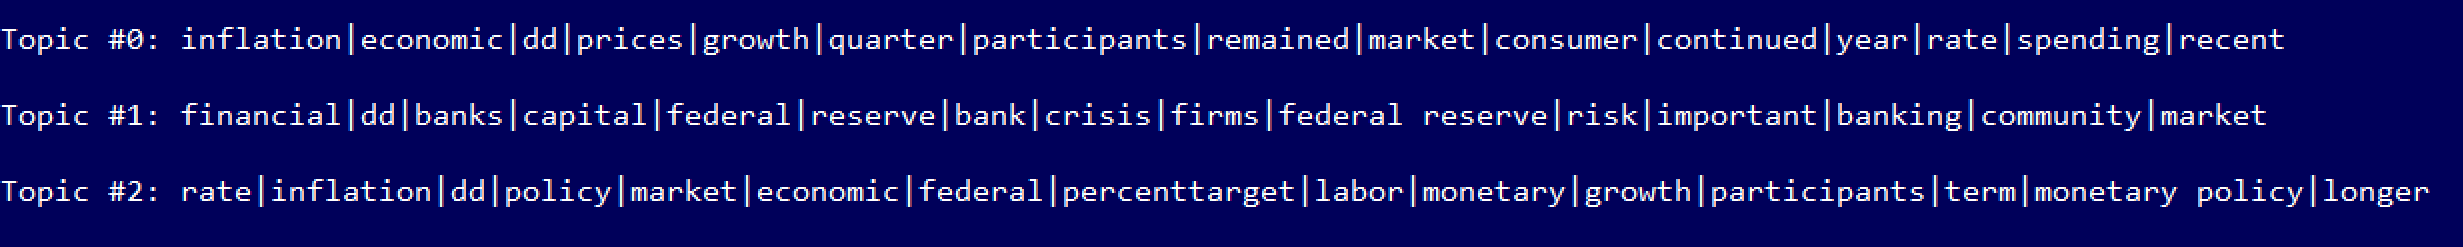
\includegraphics[width=\linewidth]{../output/data_for_graphs/Topic-Model-3-topics.PNG}
  \caption{Top 15 Words Distributed Over Three Latent Topics}
  \label{fig:LDA}
\end{figure}

We found that the topic model generally distributed the speeches and minutes into the three categories fairly well.  It was interesting that "Topic 1" referred solely to financial stability, "Topic 0" primarily referred to inflation and spending, and "Topic 2" returned a word distribution that included labor, growth, and lower for longer monetary policy. \vertSpace



% Bibliography
%-----------------------------------------------------------------
\begin{thebibliography}{99}

\bibitem{Cd94} Hansen,Stephen, McMachon, Michael  \emph{Transparency and Deliberation with the FOMC:a Computational Linquistics Approach}, CEPR Discussion Paper, (2014)

\bibitem{stanford} Puri, Indira \emph{Using Machine Learning to Predict Interest Rate Changes from Federal Reserve Proceedings}

\bibitem{nyu} Ranganath, Rajesh  \emph{NYU - CSCI-GA.2565 ML Lecture Slides Spring 2019}

\bibitem{NaiveBayes} Li, Xiang et al. \emph{The Convergence Behavior of Naive Bayes on Large Sparse Datasets}, ACM Vol 11 Issue 1, August 2016

\bibitem{LL} Zou, Yuan and Roos, Teemu \emph{Sparse Logistic Regression with Logical Features}, Helsinki Institute for Information Technology (HIIT), Springer International, 2016
\end{thebibliography}
\end{document}
